\documentclass[a4paper,11pt]{exam}
	\usepackage{graphicx}
	\usepackage[utf8]{inputenc}
	\usepackage[T1]{fontenc}
	\usepackage{listings}
	\usepackage{color}
	\usepackage{amsmath}
	\usepackage{enumerate}
	\usepackage{caption}
	\usepackage{verbatim}
	\usepackage{subcaption}
	\usepackage{tikz}
	\usepackage{pgfplots}
	\usepackage{graphics}
	\usepackage{txfonts}
	\usepackage{listings}
	\definecolor{dkgreen}{rgb}{0,0.5,0}
	\definecolor{gray}{rgb}{0.5,0.5,0.5}
	\definecolor{mauve}{rgb}{0.58,0,0.82}

	\lstset{frame=tb,
	  language=Python,
	  aboveskip=3mm,
	  belowskip=3mm,
	  showstringspaces=false,
	  columns=flexible,
	  basicstyle={\small\ttfamily},
	  numbers=none,
	  numberstyle=\tiny\color{gray},
	  keywordstyle=\color{blue},
	  commentstyle=\color{dkgreen},
	  stringstyle=\color{mauve},
	  breaklines=true,
	  breakatwhitespace=true
	  tabsize=3
	  }
	

\begin{document}
\begingroup 
	  \bf \Large Eletromagnetismo\\
	  \indent \normalsize André Del Bianco Giuffrida
	\endgroup
	\\ \quad
	\\
	\large{
	\emph{Lista 1 \\ Ex 8}
	\\
	\\
	Considere uma superfície arbitrária contendo uma densidade de carga superficial $\sigma$, em geral não uniforme.
	Demonstre as condições de contorno para o campo elétrico de cada lado da superfície: 
	\[\Big( \vec{E_1} - \vec{E_2} \Big) \cdot \hat{n} = \frac{\sigma}{\epsilon_0} \quad \text{;} \quad \Big( \vec{E_1} - \vec{E_2} \Big) \cdot \hat{t} = 0  \]
	onde $\hat{n}$ é um versor normal à superfície apontando do lado (2) para o lado (1), e $\hat{t}$ é qualquer versor perpendicular a $\hat{n}$ .
	\begin{center}
		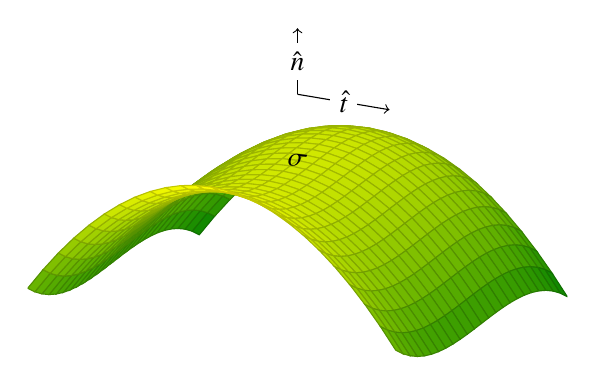
\begin{tikzpicture}
			
			\begin{axis}[axis lines=none]
			 \draw[->] (axis cs:0,0,0.5) -- (axis cs:0,0,1) node [pos=0.5, fill=white] {$\hat{n}$};
			 \draw[->] (axis cs:0,0,0.5) -- (axis cs:0.5,0,0.5)node [pos=0.5, fill=white] {$\hat{t}$};
     		 \addplot3[surf,domain=-1:1,colormap/greenyellow]{-x^2-0.3*y^3} node [pos=0.5, sloped , color=black] {$\sigma$};  ;
   			\end{axis}
   			
		\end{tikzpicture}
	\end{center}
	
	\normalsize
	Vamos começar envolvendo um pedaço da superfície com carga por uma superfície gaussiana como no desenho (cilindro com tampas):
	
	\begin{center}
		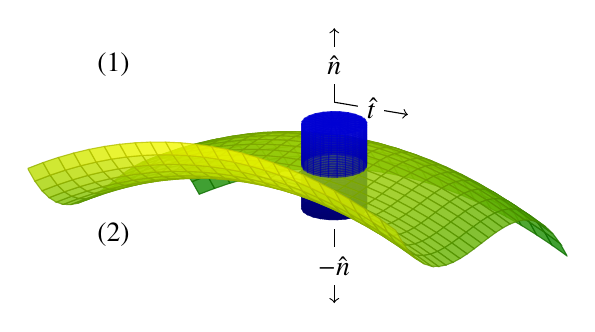
\begin{tikzpicture}
			%\draw (3,4.5) -- (3,1.5) arc (180:360:1cm and 0.25cm) -- (5,4.5) ++ (-1,0) circle (1cm and 0.25cm);
			%\draw (3,1.5) arc (180:0:1cm and 0.25cm);
			%\draw (3,1.5) arc (180:0:1cm and 0.25cm);
			\begin{axis}[axis lines=none]
				\draw (axis cs:-5,0,30) node {(1)};
				\draw (axis cs:-5,0,-50) node {(2)};
				
				\draw[->] (axis cs:1,0,30) -- (axis cs:1,0,65) node [pos=0.5, fill=white] {$\hat{n}$};
			 \draw[->] (axis cs:1,0,30) -- (axis cs:3,0,30) node [pos=0.5, fill=white] {$\hat{t}$};
			 \draw[->] (axis cs:1,0,-30) -- (axis cs:1,0,-65) node [pos=0.5, fill=white] {$-\hat{n}$};
				\addplot3[
					surf,
					domain=0:2*pi,
					domain y=0:0.8,
					shader=flat,
					opacity=0.80,
					colormap={blueblack}{color=(black) color=(blue)},
				]
                        ({y*sin(deg(x))+1},{y*cos(deg(x))},{-20});
                        
				\addplot3[
					surf,
					domain=0:2*pi,
					domain y=-20:0,
					colormap={blueblack}{color=(black) color=(blue)},
					opacity=0.50,
					shader=flat
				]
                        ({0.8*sin(deg(x))+1},{0.8*cos(deg(x))},{y});
                        
				\addplot3[surf,domain=-5:5,colormap/greenyellow,opacity=0.80]{-x^2-0.3*y^3};
			
				
				\addplot3[
					surf,
					domain=0:2*pi,
					domain y=0:20,
					shader=flat,
					opacity=0.50,
					colormap={blueblack}{color=(black) color=(blue)},
				]
                        ({0.8*sin(deg(x))+1},{0.8*cos(deg(x))},{y});
                        \addplot3[
					surf,
					domain=0:2*pi,
					domain y=0:0.8,
					shader=flat,
					opacity=0.50,
					colormap={blueblack}{color=(black) color=(blue)},
				]
                        ({y*sin(deg(x))+1},{y*cos(deg(x))},{20});
			\end{axis}
		\end{tikzpicture}
	\end{center}
	
	\[ \text{Gauss:} \quad \oint \vec{E} \cdot d\vec{a} = \int_v \frac{\rho}{\epsilon_0} dv \]
	\indent Porém a integral de $\rho$ no volume é a carga total ($Q_v$) contida no volume, sendo assim podemos calcular:
	\[\oint \vec{E} \cdot d\vec{a} = \frac{Q_v}{\epsilon_0} \quad \text{onde} \quad Q_v = \int_A \sigma da\]
	\indent Já o outro lado da integral trata do \emph{Fluxo} do campo $\vec{E}$ pelo cilindro, ao fazermos a altura do cilindro ir a zero, estaremos pegando o Fluxo nas tampas superior e inferior, ambas com area $da$, e tornaremos o fluxo sobre as paredes nulo, pois a área estará indo a zero, ou seja
	\[ \lim_{z \to 0} \oint  \vec{E} \cdot \hat{t} \, da =\lim_{z \to 0} \int_0^z  \vec{E} \cdot \hat{t} \, 2 \pi \, z' \, dz' = 0 \]
	\indent Mesmo que o campo tenha componentes na direção $\hat{t}$ a área vai a zero $ \quad \therefore \quad $ Fluxo de $\vec{E}$ por uma área nula é nulo. \\
	
	\[\int_{A_1} \vec{E_1} \cdot \hat{t} \, da + \int_{A_2} \vec{E_2} \cdot (-\hat{t}) \, da = 0 \quad \text{onde} \quad \Big(\vec{E_1}\cdot\hat{t} + \vec{E_2}\cdot(-\hat{t})\Big) \, da = 0\]
	\indent Então o Fluxo total fica:
	\[\oint \vec{E} \cdot d\vec{a} = \int_A \frac{\sigma}{\epsilon_0}\, da \]
	\[\int_{A_1} \vec{E_1} \cdot \hat{n} \, da + \int_{A_2} \vec{E_2} \cdot (-\hat{n}) \, da = \int_A \frac{\sigma}{\epsilon_0}\, da \quad \text{onde} \quad \Big(\vec{E_1}\cdot\hat{n} + \vec{E_2}\cdot(-\hat{n})\Big) \, da = \frac{\sigma}{\epsilon_0}\, da\]
	e Assim chegamos as condições de contorno :
	\[ \Big( \vec{E_1} - \vec{E_2} \Big) \cdot \hat{n} = \frac{\sigma}{\epsilon_0} \]
	\[ \Big( \vec{E_1} - \vec{E_2} \Big) \cdot \hat{t} = 0 \]
	
	\begin{figure}[h]
		\centering
		%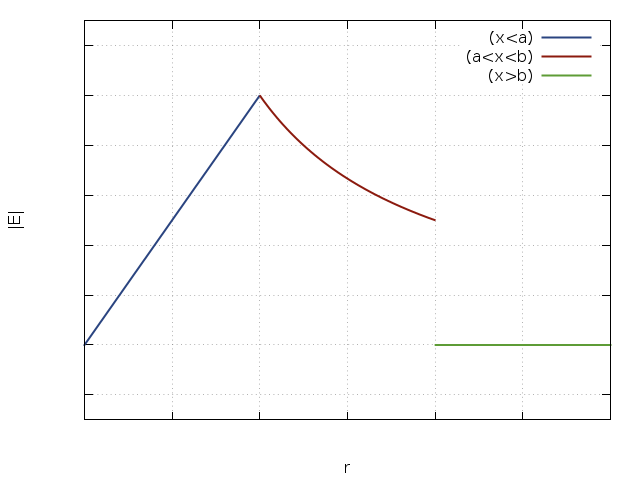
\includegraphics[scale=0.6]{Ex.png}
		%\caption{ $| \vec{E}(\vec{r}) |$ nas três regiões}
	\end{figure}
	
\end{document}
